\documentclass{article}

\usepackage{csquotes}
\usepackage[margin=0.7in]{geometry}
\usepackage{graphicx}

\title{FPGABoy Documentation}
\author{Luke Wren}

\begin{document}

\pagenumbering{gobble}
\maketitle
\tableofcontents
\newpage
\pagenumbering{arabic}

\section{What?}

FPGABoy is...
\begin{itemize}
\item An open source games console
\item An open source PCB layout
\item Designed with KiCAD open source PCB editor
\item An open source CPU, graphics and bus architecture
\item Based on the RISC-V open source instruction set
\item Synthesised and taped out with iCEStorm open source FPGA toolchain
\end{itemize}

\begin{displayquote}
\textit{If you say open source one more time I swear I'm gonna nut instantly} - Oscar Wilde
\end{displayquote}

\subsection{PCB}

The board is a 4-layer stackup:

\begin{enumerate}
\item Signal + GND Fill
\item GND plane
\item Power planes
\item Signal + GND Fill
\end{enumerate}

It is intended to be suitable for low-cost PCB prototyping services such as iTead. Board dimensions are 50mm $\times$ 50mm, which fits into the cheapest size category on iTead. For the most part, it sticks to the following minimum specifications:

\begin{itemize}
\item Track width 0.15mm
\item Copper-copper clearance 0.15mm
\item Soldermask-copper clearance 0.1mm
\item Soldermask width 0.1mm
\item Via drill 0.3mm
\item Annular ring 0.15mm (i.e. via diameter 0.6mm)
\end{itemize}

The only exception is some 0.5mm vias underneath the BGA. Strictly this is out of specification for iTead, but they claim to have a 90 $\mu$m drill registration, so we'll see how it goes.

The iCE40-HX8k FPGA is packaged in a 256-pin 0.8mm BGA, which \textit{can be} reflowed by a hobbyist with a hot air gun or a frying pan (best to choose a HASL finish so that contacts are pretinned). The 132-pin 0.5mm BGA has sufficient IO for our needs, but iTead does not manufacture at the tolerance required for such a fine pitch.

\subsection{Logic Design}

The heart of the design is a Lattice iCE40-HX8k FPGA, containing 7680 LUT4s and flipflops. The logic was designed from scratch, using synthesisable Verilog. This includes:
\begin{itemize}
\item RV32EC-compatible 32-bit CPU design
	\begin{itemize}
	\item E: embedded profile (reduced register set)
	\item C: compressed instruction extension, for higher code density
	\end{itemize}
\item Graphics pipeline
	\begin{itemize}
	\item Don't expect much, it's about as powerful as a Gameboy Advance
	\item Includes some MODE7-like functionality which allows drawing perspective-mapped textured planes, by providing per-scanline affine texture transformation. Think MarioKart
	\end{itemize}
\item AHB Lite 3.0-compatible multi-master busfabric
\item Other peripherals
	\begin{itemize}
	\item External SRAM controller
	\item Display controller
	\item DMA master
	\item Interrupt controller
	\item GPIO controller (buttons!)
	\item Serial port etc.
	\end{itemize}
\end{itemize}

Some attempt is made in this document to describe the operation of these hardware blocks, but if you are looking for nitty-gritty detail, the best documentation is the files ending with \texttt{.v}.

That a free synthesis tool can cram all this logic into one of the cheapest FPGAs on the market is tremendously impressive. Hopefully we will one day have a situation similar to software compilers, where free tools such as GCC are industry standards.

\section{CPU Architecture}

\begin{figure}[!htb]
\caption{ReVive architectural block diagram}
\centering
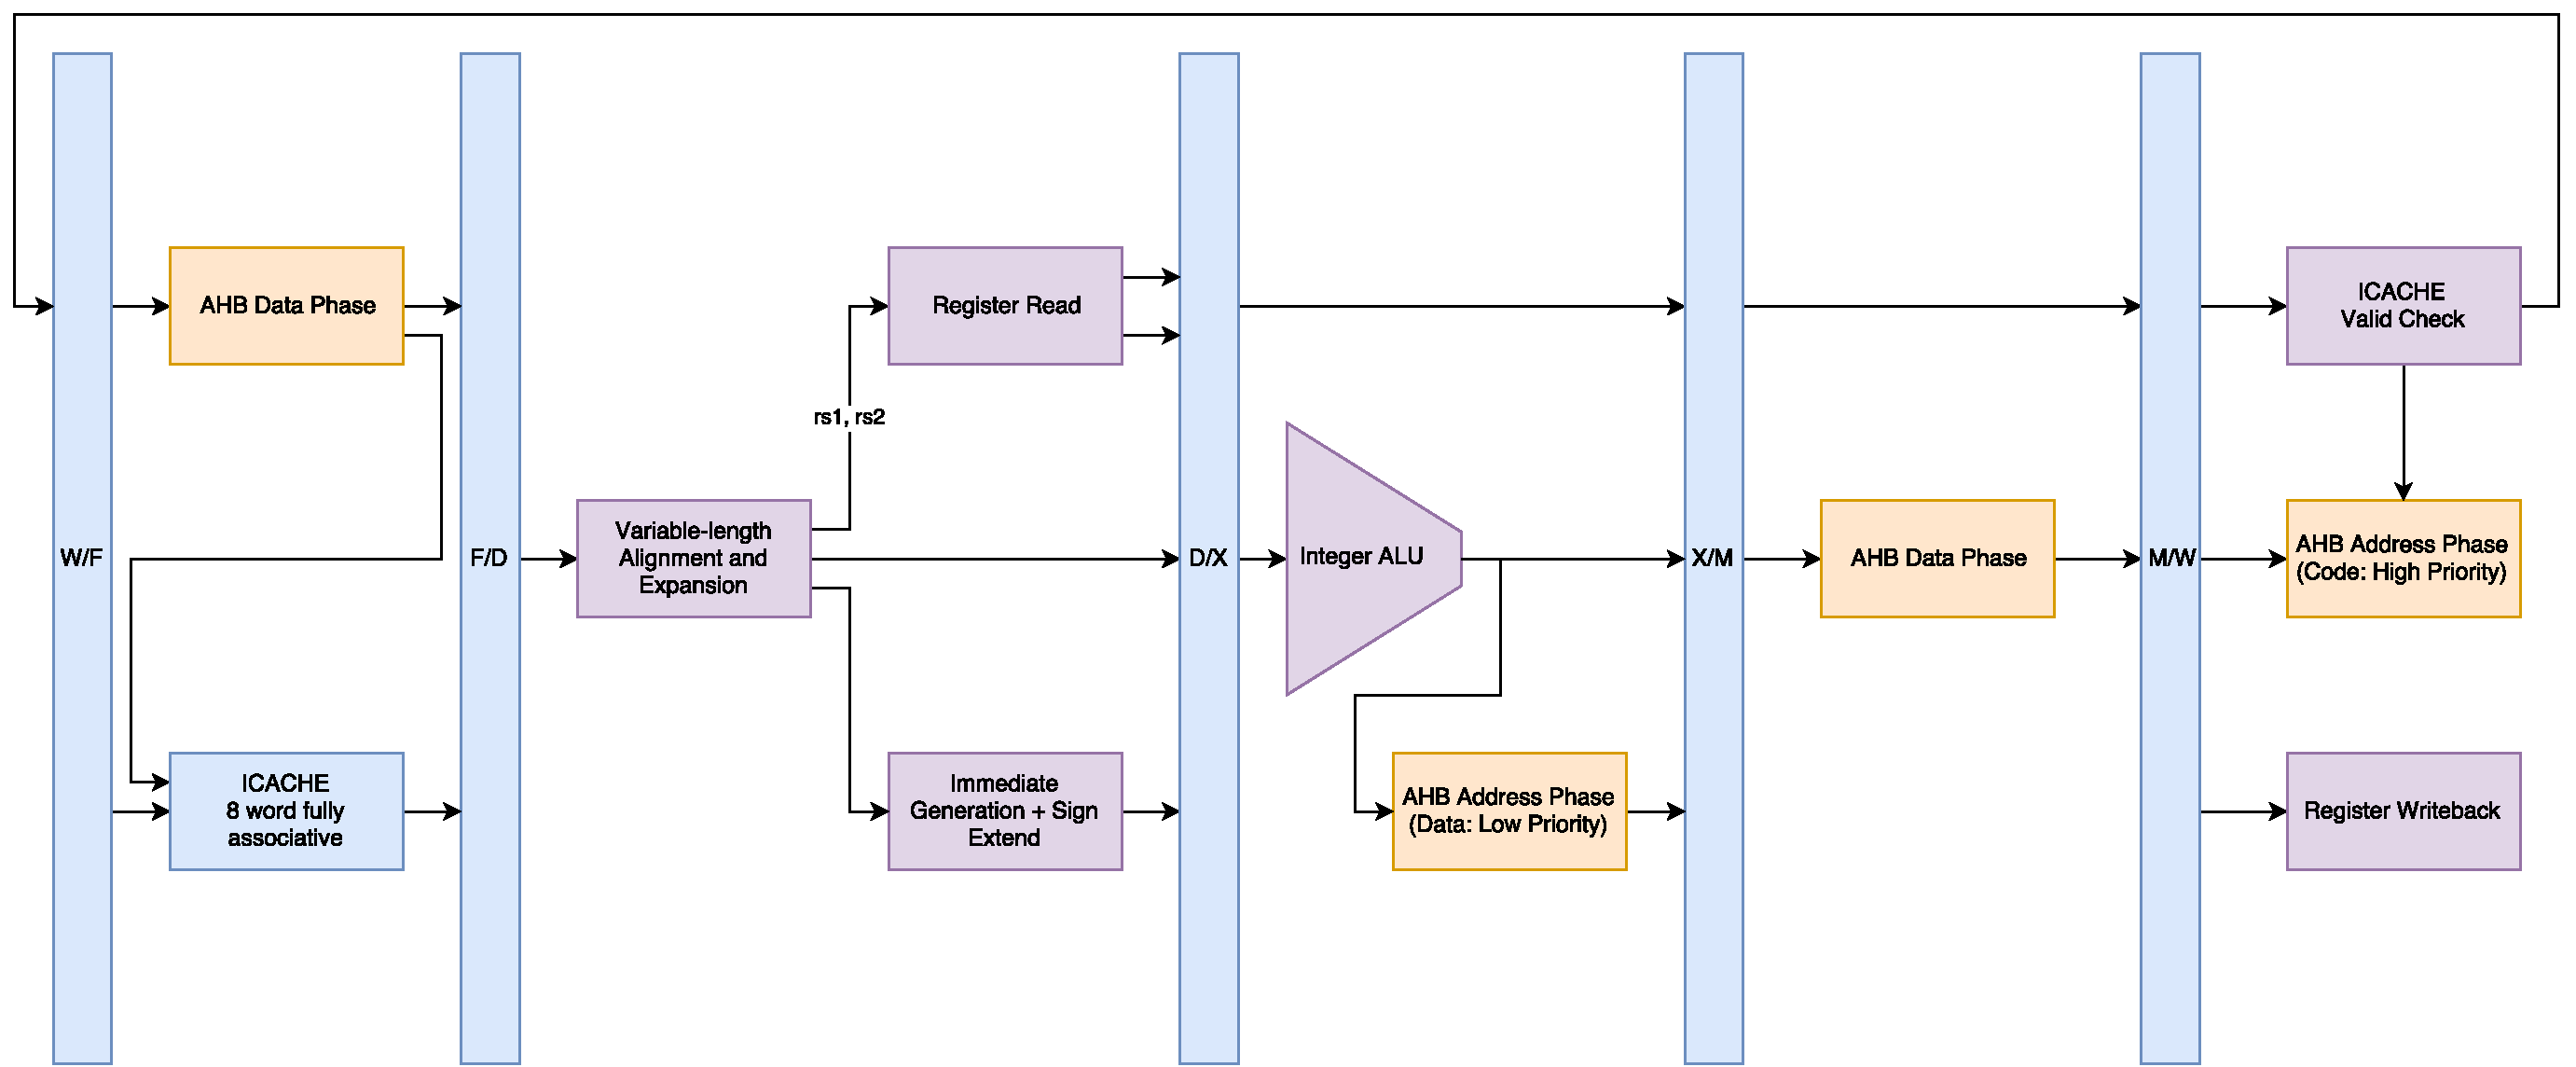
\includegraphics[width=0.9\textwidth]{diagrams/cpu_block.pdf}
\end{figure}

ReVive is a 32-bit processor based on the RISC V (hereafter RV) instruction set architecture. The name seemed appropriate for what is supposed to be a return to the glory days of games programming, when NULL pointers were just pointers to the start of ROM, and programmers were real programmers who wrote their \textit{own} polygon rasterisers, dammit.

The diagram shown here is a simplified block diagram of the core. Not shown is:
\begin{itemize}
\item The full and specific contents of the pipeline registers
\item The forwarding/bypass network which shortens data hazards to improve pipeline throughput
\item Additional hardware in ICACHE which helps to support unaligned code fetches
\item Interrupt entry/exit hardware
\item The ready/valid handshakes on pipe stages which allow them to NOP later stages, and stall prior ones
\item Hardware registers such as PC, and PC update logic
\item Pipeline flushing signals for branch mispredict
\end{itemize}

Overall this is a fairly standard RISC-style processor pipeline. The tall blue boxes represent the registers at the boundaries of two pipe stages. The nomenclature used in the diagram is:

\begin{itemize}
\item F: fetch
\item D: decode
\item X: execute
\item M: memory access (load/store)
\item W: register writeback
\end{itemize}

The processor has a single AHB-lite busmaster; the instruction fetcher and the load/store stage need to share it, and the instruction fetch takes priority.

Branches are speculated, according to the static prediction scheme described in the RV ISA manual:

\begin{itemize}
\item Backward branches are predicted to be taken, on the assumption that loops will run at least twice on average.
\item Forward branches are predicted not taken; the ISA manual advises that compilers should put more likely code on this path.
\end{itemize}

RISC-V compressed instructions achieve respectable code density, but it's no Thumb-2. The instruction cache helps to tame the fetch bandwidth, so that load/stores and other system masters will still see some appreciable fraction of the bus bandwidth.

\end{document}